\section{Maximum Intensity Projection}\label{Sec:Mip}
\subsection{Tri-linear interpolation}
The method to determine the voxel of a position that was used in the skeleton code was the nearest neighbor technique. 
That is, find the nearest position that has a known Voxel value and use that value. 
Tri linear interpolation uses the technique of interpolation in three dimensions.

It works as following in one dimension. 
Suppose we know that we get 5 coupons when we buy 20 items and 20 coupons when we buy 30 items. 
Then we can guess how many coupons we would get when buying 22 items. 
We can do that in this way: $((30-22)*5 + (22-20)*15)/(30-20) = 7$ 
So we would guess that we would get 7 coupons, when buying 22 items.

We can do the same for three dimension, by doing this step by step. 
We can first interpolate in the x dimension , then in the y dimension and finally in the z dimension.
To do this we need the 8 surrounding points, that know their voxel. 
Suppose we want to know the value of $X_{a},Y_{b},Z_{c}$. 
Then we round down a,b,c to i,j and k. 
We then have the surrounding points: $(X_{i},Y_{j},Z_{k}), (X_{i},Y_{j}, Z_{k+1}), (X_{i},Y_{j+1},Z_{k}),
 (X_{i},Y_{j+1},Z_{k+1}), (X_{i+1},Y_{j},Z_{k}), (X_{i+1},Y_{j},Z_{k+1})$, \\ $ (X_{i+1},Y_{j+1},Z_{k}) , (X_{i+1},Y_{j+1},Z_{k+1})$.
 
We can use this values to estimate the values for the x-axis. 
We can do this in the same way as we did with one dimensional interpolation. 
We take xd = (a-i) , because i+1 - i is always 1.
We already do the same for y and z: yd = (b-j), zd = (c-k) 
Then for each combination where the y and z are the same, but the x differs we can compute their new approximates: \\
$c00 = xd(X_{i},Y_{j},Z_{k})+(1-xd)(X_{i+1},Y_{j},Z_{k})$ \\
$c01 = xd(X_{i},Y_{j},Z_{k+1})+(1-xd)(X_{i+1},Y_{j},Z_{k+1})$ \\
$c10 = xd(X_{i},Y_{j+1},Z_{k})+(1-xd)(X_{i+1},Y_{j+1},Z_{k})$ \\
$c11 = xd(X_{i},Y_{j+1},Z_{k+1})+(1-xd)(X_{i+1},Y_{j+1},Z_{k+1})$ \\
Then we only have four points left. We can then do the same for the y-axis and then we only have two points left. \\
$c0= yd(c00)+(1-yd)(c01)$\\
$c1= yd(c10)+(1-yd)(c11)$\\
Finally we can do the same for the z-axis and then we have computed the voxel for the point we were interested in.\\
$c= zd(c0)+(1-zd)(c1)$\\
Which is the value we are looking for. 
In figure~\ref{fig:interpolation} you can see a small difference between the first and second tomato.
The second tomato has beter aliasing and less noise around the kernels. 
However the slicer without tri-linear interpolation is a lot faster. 

\begin{figure}[H]
	\centering
	\begin{subfigure}[t]{0.45\textwidth}
		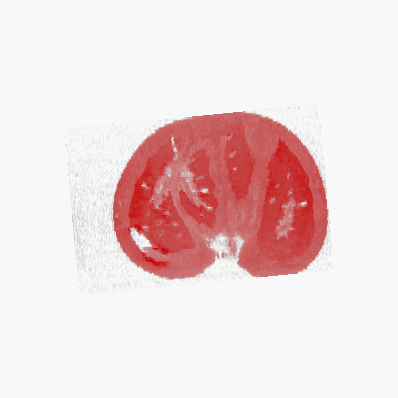
\includegraphics[width=\textwidth]{tomato1}
		\caption{Rendering with slicer and tri-linear interpolation disabled}
	\end{subfigure}
	~%
	\begin{subfigure}[t]{0.45\textwidth}
		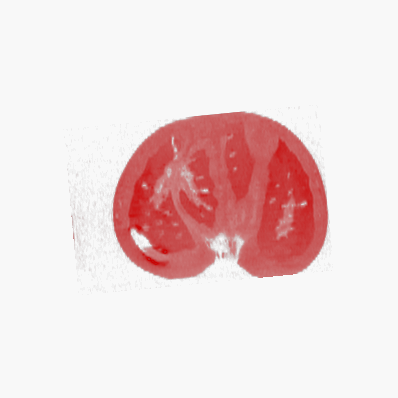
\includegraphics[width=\textwidth]{tomato2}
		\caption{Rendering with slicer and tri-linear interpolation enabled}
	\end{subfigure}
	\caption{A comparison of rendering \texttt{tomato.fld} with and without tri linear interpolation}
	\label{fig:interpolation}
\end{figure}

\subsection{Maximum Intensity Projection}
Maximum intensity projection, projects the point with the largest voxel along the viewing ray. 
So we adjusted the slicer method that it looks at all points along the viewing ray and not just the point of that slice. 
We can do this by simply adding another loop after the loop for each pixel. 
Then we save the value if it is bigger than all previous values, so we know the maximum voxel value.
We do this for each viewing ray and use the same color function as the slicer. 
This is how we implemented the maximum intensity projection.

This works really slow in combination with Tri-linear interpolation.
A suggested method to quicken the maximum intensity projection was to change the resolution. 
We will describe this in the next subsection. 
Another method we used was to render the image in another thread, so we could still use the GUI.
We will desribe this in Subsection~\ref{Sec:Perf:Background} on background rendering.
